
\documentclass{article}


\usepackage[square,numbers]{natbib}
\usepackage{amsmath, epsfig}
\usepackage{amsfonts}
\usepackage{subfigure}
\usepackage{graphicx}
\usepackage{amsfonts}
\usepackage{algorithm}
\usepackage{algorithmic}
\usepackage{easybmat}
\usepackage{footmisc}
\usepackage[usenames,dvipsnames]{color}
\usepackage{subfig}
\renewcommand\algorithmiccomment[1]{// \textit{#1}}
\newcommand{\ignore}[1]{}
\newcommand{\comment}[1]{}
\newcommand{\frank}[1]{\textcolor{red}{\textsf{\emph{\textbf{\textcolor{blue}{#1}}}}}}
\newcommand{\willie}[1]{\textcolor{green}{\textsf{\emph{\textbf{\textcolor{green}{#1}}}}}}
\DeclareMathOperator*{\argmax}{arg\,max}


% need to include style sheet for journal



\begin{document}


\title{Unsupervised Detection and Tracking of Multiple Objects with Dependent Dirichlet Process Mixtures}
\author{Willie Neiswanger and Frank Wood}
\maketitle
\mbox{}

\abstract{main points}



\section{Introduction}

\frank{this section should introduce our work and situate it relative to the literature}
\willie{okeydoke. this isn't ready yet. to avoid confusion I've just commented the whole section out.}


% % \subsection{Topic Overview and Terminology}

% This work is related to the study of algorithms that perform automated detection and tracking of arbitrary objects in videos; we define such algorithms as those with the ability to decide which spatiotemporal regions of a video constitute objects (extraction), find the positions and/or shapes of distinct objects (localization), and maintain the positions of the detected objects over time (tracking). Robust algorithms which can carry out these tasks are applicable to problems in the fields of surveillance, autonomous systems and robotics, and video summarization and compression. Approaches to these tasks have been proposed under different headings and in a variety of contexts. This section serves to introduce relevant terminology and topics of research.

% The task of extraction is closely related to the topics of foregound segmentation, background modeling, motion detection, and appearance feature extraction. In general, these methods aim to extract features from regions of a video frame that are considered objects or are distinguished in some way from the background of a scene. Areas of research in this field include attempts to handle situations where the background displays motion or other dynamic characteristics, reduce noise caused by the false extraction of backgrounds, handle abberant image effects present in some videos, and operate accurately on scenes involving illumination changes.

% The task of localization is closely related to the topics of object detection, position-finding, target segmentation, contour-detection, template matching, and recognition. These methods are mainly concerned with finding the positions and/or shapes of objects in a given video frame, or with discerning between objects similar in position or appearance. There has been a focus in this field on developing techniques for representing an object's appearance, both to allow for localization of objects on a per-frame basis and to allow for consistent localization of a given object over time. Research into the unsupervised detection of arbitrary objects (which we define as methods that accomplish both extraction and localization) has included work involving image segmentation, parsing, and pixel clustering. These topics usually relate to the automated partitioning of images into meaningful regions. Note that the popular phrase `object detection' is also typically used to refer to procedures that carry out extraction and localization; however, it is often reserved to denote methods that are tailored to find the position of specified objects or object types (as opposed to arbitrary object detection), or to denote supervised methods, where extraction is peformed implicitely during searches for specified objects and localization procedures.

% The task of tracking is closely related to the topics of video tracking, data association, filtering, point matching, and `tracking of non-rigid objects'. In general, these tasks aim to maintain localization of the positions and/or shapes of objects over time. Areas of interest in this field involve developing metrics for judging the similarity between two object representations (for example, potential representations of the same object at adjacent frames in a video), techniques that provide a way to conduct efficient searches over a frame for regions that are similar to a given object, and methods for predicting the future position or appearance of an object. A great deal of research in this field over the past decade has focused on the development of algorithms to track multiple objects simultaneously. There has been a particular emphasis on developing ways to deal with problems such as object occlusions (where one object blocks another from the view of a video camera), complex object interactions, object coalescence (where one object is tracked by multiple times/redundantly), objects with similar appearances, variable (and potentially high) numbers of objects, and objects that enter and exit a field of view at different times.

% There does not yet exist a major body of research concerned primarily with methods for combining extraction, localization, and tracking to perform cohesive unsupervised detection of arbitrary objects in videos. Many papers that attempt to accomplish this goal focus on one of extraction, localization, or tracking, and attempt to integrate in methods from the other two tasks. However, a few key schemes for unsupervised detection and tracking do indeed exist. A widely applied, though unsophisticated, technique to carry out such a procedure is called blob tracking. Blob tracking typically refers to methods that perform extraction and localization at each frame independently--for example, by assuming that object pixels have a different intensity than background pixels, setting a fixed pixel intensity threshold for extraction of object pixel locations, and segmenting the extracted data into `blobs' to accomplish localization. Afterwards, tracking is often carried out by finding the centroid of each blob and applying standard multiple target tracking algorithms (described in [section]). Note that blob tracking carries out the three main tasks described above, so it satisfies the criteria for the type of unsupervised detection and tracking algorithms studied in this work; there are, however, many challenges associated with blob tracking that render it impractical in many settings (detailed in [section]).

% This paper presents a new method for unsupervised multiple object detection and tracking. We introduce, and provide details on the theory behind, a technique involving dependent Dirichlet process mixture models. Specifically, this work applies the model to data gained during the extraction process; note that data of this type is refered to at different points in the paper as `extraction data', `data points', 'points', or 'observations'. The model is first presented in an abstract form, which could be adapted to a wide range of extraction procedures and object appearance representations (mainly left for future studies). We then describe inference algorithms that allow object localization and tracking to be carried out. Afterwards, we formulate a definite model for data gained during a specific extraction procedure and implement the described inference procedures to carry out multiple object detection and tracking in a number of experiments.


% \subsection{Related Work}

% Related work can be broken down into studies relating to extraction procedures, unsupervised localization procedures, single object tracking methods, multiple object tracking methods, supervised multiple object detection and tracking methods, and unsupervised multiple object detection and tracking methods.

% Extraction procedures can usually be classified as either model-based methods or heuristic-based methods. Model-based methods emphasize the detection of shapes of regions containing objects accurately and reducing background noise. For example, foreground extraction has been robustly carried out by modeling each pixel over time in order to infer a probability distribution over pixel values; if the pixel takes on a very unlikely value at a future time, it is marked as a foreground pixel at that point \citep{stauffer_1999, elgammal_2000, elgammal_2002}. These pixel modeling techniques have been adapted to allow for time-dependent probability distributions over pixel values, which help account for slighlty changing backgrounds, such as those caused from brief movements of background objects (for example, trees in outdoor scenes). Note that these techniques treat each pixel independently; this has a tendency to cause errors in foreground detection, resulting in fragmentation of foreground images (which is problematic as many of these methods intend to blob the foreground objects after detection in order to perform segmentation and locate objects' centroids). Post processing has been applied to add information regarding the edges of objects in an attempt to decrease fragmentation \citep{turdu_2007}. Others have attempted to achieve better foreground modeling in cases where the foreground and background exhibit similar color distributions (the so called `color similarity problem') by, for example, incorporating models of the foreground into a typical background model (such as the one described above) \citep{gallego_2009, mchugh_2009}.

% On the other hand, heuristic-based methods perform extracting by looking for temporal changes in pixel value characteristics. While these methods locate regions with objects less accurately than model-based methods, they are often much less computationally expensive. Frame differencing and background subtraction are two such methods, and involve comparing pixel values, or groups of pixel values, between two images, to detect a change surpassing some threshold. The goal of these techniques is to find locations in a scene that display motion, and to deem these moving areas the foreground of a scene.  Often, background subtraction refers to comparing an image containing targets with an image of the background without targets or with some model of the background that is learned as the video progresses (in these cases, objects that do not move throughout a scene will be treated as the background), while frame or image differencing refers to comparing two subsequent images in a video. Frame differencing has been used as the sole extraction method for object localization or tracking schemes with success \citep{pece_2002, beleznai_2006, chu_2007}, and also as a secondary data extraction method to help improve the accuracy of object tracking schemes \citep{perez_2002}. In addition to the two techniques mentioned above, there exists other ways of extracting movement from an image, such as through techniques involving optical flow (a calculation based on a so called `generalized gradient model' of an image, which attempts to capture the speed and direction of movement over areas in the image) \citep{horn_1981, bobick_2001}. In \citep{black_2000}, a motion detection and object tracking method is developed based on the relative motion of moving objects' boundaries, which are again found through analysis of optical flow.

% There are an extensive collection of methods for tracking single, non-rigid, objects. For example, color has long been used for tracking. In this case, tracking refers to the task of maintaining the location of an object after its initial position has been specified. In general, these schemes operate by modeling an object with some color-based appearance model, and using this model to find the object in subsequent frames. One classic approach involves modeling the color of a target (in particular, a distribution over the hue-saturation space of a target region) with a Gaussian mixture model (GMM), and choosing subsequent target positions by searching surrounding areas for regions that yield similar GMMs. Furthermore, the GMM is often allowed to adapt over time, and slowly change to model changes in lighting or other smooth time-based variations in the target's color \citep{raja_1998, mckenna_1999, jepson_2003}. Others have attempted to abstract this work with a non-parametric color modeling approach based on kernel density estimation, which does not assume a specific underlying distribution (such as the Gaussian mixture in the previous case) and instead converges to reasonable distribution that depends on the data \citep{elgammal_2001}. Additionally, color has been successfully applied as the feature in the mean-shift procedure (kernel-based method) for tracking \citep{comaniciu_2003, perez_2002, nummiaro_2003, lee_2011}.

% The mean-shift procedure (also known as `kernel-based object tracking') attempts to provide a robust way for non-rigid objects to be tracked. This method is beneficial because it optimizes the search for the `next' position of an object (i.e. the search for the region in a frame which is most similar to a target region in the previous frame). This procedure--a derivation and overview of which can be found in \citep{fukunaga_1975, cheng_1995}--involves an iterative algorithm that repeatedly shifts each data point to the weighted average of data points in its neighborhood; it has been proven that this process converges for each data point. Additionally, the process (in particular, the specification of the neighborhood and the weight-distribution when calculating the weighted mean of nearby data points) is generalized so that multiple kernels can be specified and used to allow for varied clustering behaviors. It can be shown that, through this procedure, each data point becomes associated with a local point of high density (dependent upon the underlying weight distribution specified by the kernel) which naturally allows for clustering \citep{cheng_1995}. The mean shift algorithm has been implemented successfully to allow for a sort of kernel-based object tracking \citep{comaniciu_2003, comaniciu_1999, comaniciu_2000}. Given the current position of an object at a given frame, the goal of tracking is often to find a nearby position in the next frame that has the most similar distribution over some common set of features. Usually this must be done through an exhaustive search, comparing the similarity of distributions at each nearby position with that at the current position. However, if a certain type of `isotropic kernel' (mean-shift kernel) known as the Bhattacharyya coefficient is chosen as a similarity metric between the feature distributions at two positions, it creates a smooth function where gradient descent techniques can be used to quickly converge upon an optimal subsequent position without using an exhaustive search. Many papers are concerned with applying this kernel-based object tracking scheme to different sets of features or with different kernels. Additionally, the scheme has been attempted with an adaptive kernel whose shape, scale, and orientation is influenced by a target being tracked \citep{wang_2004}, with a kernel adjusted by the estimated centroid of a tracked target \citep{mehmood_2009}, and with a heirarchical version of the mean-shift procedure \citep{dementhon_2002}. 

% Some have tried to extent single object tracking schemes to tracking multiple targets; at the most basic level, this involves initializing multiple targets and running an instance of (single) VOT for each, either simultaneously or in succession \citep{perez_2002}. Furthermore, if performed simultaneously, the tracking of each target can be made dependent upon characteristics of other targets (such as their proximity) to resolve errors and improve tracking (such as those caused by the incorrect merging of two targets) \citep{khan_2004, vermaak_2003} . 




% %  ------------------------------------------------------------------------------------
% % Localization-focused. Clustering methods, segmentation methods, object appearance models and representations (allows for consistent object localization over time).

% % Methods for tracking single objects in videos: filtering, similarity metrics / localization (and how they play a role), mean shift procedures.

% % extensions to multiple visual object tracking. problems with multiple independent single object trackers (coalesence, object interaction, object occlusion, objects entering and leaving scene [and, relatedly, variable numbers of objects]).
% % Multiple object tracking attempts at overcoming various the various challenges specified above (include nonparametric varmaak/doucet for maintaining multi-modality here?---sure, and then mention again later with fox's work?)
% % End with description of initialization problem.

% % Methods for detection and tracking of objects. Heuristic initialization at beginning and then carrying out above methods (problems with varying numbers of obects / objects entering or leaving scene). Supervised learning of specific targets to allow for initialization and provide better localization throughout. Various research has been towards integrating unsupervised extraction and localization into multiple object tracking methods. Particle filters with integrated detection (at least two of these). Introduce concept of blob tracking and define basic algorithm (some manner of extraction, independent/per-frame localization, tracking; note that each object is represented in each frame as a low-dimensional point [or higher dimensional thing like region/outline with sophisticated blob/contour detectors like bramble and others]). The key thing characterizing a blob detector is that the position of each object (or the spatially separate region associated with each object) is assigned/fixed at each frame without the aid of tracking (ie if localization/segmentation can be carried out at each frame independently), and tracking is done with this data. Schemes often are simply segmentation of extraction data into spatially disjoint blobs at each frame (where blobs  are not modeled in any principled manner), returning the position or region associated with each object at each frame.

% % When the state of objects (for example, position and/or other characteristics) can be found independently at each frame, well established methods in the field known as Multiple Target Tracking (MTT) can be carried out to perform tracking of multiple objects. Two classic algorithms for MTT are known as MHT and JPDA. In general, MTT methods are useful for procedures that can represent each object at each frame as a point or region without localization information from this object at a previous frame (which requires the use of tracking). MTT in the literature is often quite separate from fields of computer vision involving object detection and tracking research. In general, the situation arises as video data without modification is very high dimensional (discussion of difference between MTT and detection methods here?).


% % Methods like blob tracking which attempt to find the state of each object independently at each frame have a hard time dealing with occlusion and other complexities (except for sophisticated blob trackers like bramble which isn't really blob tracking). Attempts have been made to perform time dependent clustering on extraction data (look at cluster tracking paper for good def), to carry out joint localization and tracking; this has been refered to as cluster tracking. Work of Pece, MTT of multiple targets work(?). The work presented in this paper most closely resembes the topics listed here. Does cluster tracking on whichever extraction data, using a time dependent Dirichlet Process mixture model (to better estimate and maintain the number of targets, as was shown to be effective in vermaak and fox), which takes the form of a sequence of clusters, where the objects' appearances are modeled in a principled manner by the cluster component distributons, and the tracking behavior is modeled by time-dependencies between adjacent elements in the cluster-sequences.
% %  ------------------------------------------------------------------------------------




% \subsection{Contributions}

% This paper applies a time dependent Dirichlet process mixture to model data gained during extraction procedures, provides background as to how this Bayesian nonparametric model allows for the incorporation of prior knowledge about object appearances and motion behaviors, describes methods for unsupervised detection and tracking of arbitrary objects in terms of Bayesian inference procedures, and presents a specific implementation of the model and inference procedures to carry out detection and tracking on a number of target-types in different settings.

% % List here the benefits of this idea that should be discussed/listed:
% This paper is heavily model-based, which differs from many papers in the field of multiple object tracking that do not explicitely describe models which underlie various procedures that are carried out. Solutions in many papers are, instead, algorithm oriented. The model-based approach allows rigor to be kept as inference procedures are developed. Furthermore, development of inference procedures are performed separately from development of the model, and various well studied inference and approximate inference methods can be carried out to achieve algorithmic results that are (in some cases) known to be optimal.
% %treated separately, which allows for multiple methods to be carried out in a unified framework and   these solutions are  but provide algorithm-based presentations.
% %	This way allows rigor to be kept as inference procedures are developed.
% %	Furthermore, inference is treated separately; this allows multiple detection and tracking algorithms to be developed (in a well-formed/rigorous fashion) by developing different inference techniques. Also, inference on graphical models is a well-structured field and allows for use of techniques in this field as well as better interpretations of the resulting detection/tracking algorithms.
	
% % (related to previous?) models objects as distribution-components (of a mixture model) as opposed to point-targets or targets with noise that adheres to some distribution (is this truly a distinction and is it good?)



% This idea presents a framework which allows for time-varying models of objects' appearances and motion behaviors to be incorporated, and is formulated in a Bayesian manner that allows distributions underlying the parameters of these models to be specified in a principled manner. It has been shown to work successfully in conjunction with simple (noisy) extraction methods. More robust, expensive, or in general accurate methods can be used for further accuracy. This method is able to handle the appearance and disappearance of objects from a scene, variable numbers of objects, cases where objects show time varying changes in behavior, and cases of occlusion.

% Section two of this paper provides an overview of the model and describes how aspects can be modified for for modeling object appearance and motion behavior. Section three presents a specific implementation of the model and a number of inference procedures for carrying out object detection and tracking. Section four describes a number of experiments carried out with this implementation. Section five describes results of these experiments, comments on further directions of study, and provides concluding remarks.













\section{Model Overview}
\label{sec:modeloverview}
%
This section provides details on the nature of the data to be modeled, Dirichlet process mixture (DPM) models, and dependent Dirichlet process mixture (DDPM) models. We end by making explicit the connection between elements of the model and object characteristics that these elements represent (for example, the appearance and motion behavior of objects are specifically captured). The provided model is formulated here in a sufficently abstract manner to allow for various representations of objects to be specified in future studies.




\subsection{Data}
\label{sec:data}
%
We defined the task of extraction to be the unsupervised decision of which spatiotemporal regions of a video constitute objects; hence, the extraction data modeled in this work are D-dimensional observations that in some way provide information about the regions of the video frame that contain objects. A simple example of this information is shown by the three-dimensional extraction data $\bold{x} = ( x_{1}, x_{2}, t ) \in \mathbb{R}^{2} \times \mathbb{Z}_{+}$, where $x_{1}$ and $x_{2}$ are the two spatial dimensions of pixels contained in regions comprising objects in a given frame, and $t$ is the discrete time index of the frame. These three features are always available once regions containing objects are discerned, and should always be kept as features of the data for modeling (as position information is key for reasonable tracking and time information is necessary for our intention to model the temporal dependencies of the data).

Examples of additional features that could potentially be extracted from video frame regions containing objects include color information, pixel intensity values, feature point (such as corner, shape, or edge) locations or spatial characteristics, texture representations, transform results (such as results of hough or fourier transforms), and quantiative region descriptions derived from image segmentation procedures; the main idea is to choose features which are able to be easily extracted or computed, capture variability in the appearance of objects, are applicable to a wide variety of object types, and, when viewed in cumulation for multiple observations, are distributed in a way that allows for modeling and tractable inference (this is discussed further in section 3).

We will use the phrase `baseline' three-dimensional extraction data to refer to the $\bold{x} = ( x_{1}, x_{2}, t ) \in \mathbb{R}^{2} \times \mathbb{Z}_{+}$ from pixels present in regions containing objects. These data are distributed roughly as worm-like shapes that follow the paths of individual objects as they move, when they are plotted in three dimensions (where we let the frame number, our discrete representation of time, ascend the vertical axis and the spatial positions occupy the horizontal axes). An example of data with such a distribution can been seen in Figure 1. The data consists of the three-dimensional baseline features and was gained by extraction peformed on a 50 frame sequence showing five ants moving across the video scene.
\begin{figure}[h]
        \center{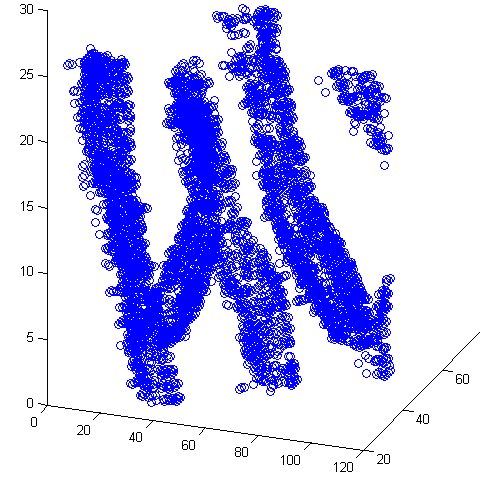
\includegraphics[width=75mm]{paths.png}}
        \caption{\label{Figure 1:} Baseline three-dimensional extraction data gained from a video of multiple moving targets. The vertical axis denotes the frame number and the horizontal axes denote $d_{1}$ and $d_{2}$ spatial coordinates, respectively, of pixels within a given frame. The data comes from a 50 frame video segment showing 5 moving ants (note that one ant enters the scene near the middle of the segment).}
\end{figure}
Inference performed on the time dependent Dirichlet process mixture model (described in the following sections) carries out clustering of the data, which allows each worm-like data cloud to be isolated and independent objects to be localized and tracked.






\subsection{Dirichlet Process Mixtures}

Dirichlet process mixtures fall under the heading of Bayesian nonparametric (BNP) models. These models have been widely used over the past decade to perform nonparametric density estimation and cluster analysis. They are, in particular, useful for estimating the number of latent classes (clusters) in mixture models. In this work, estimating the number of clusters in the data generated via extraction is shown in the following sections to be equivalent to estimating the number of distinct objects in a video. Consequentially, a model which is able to perform robust nonparametric estimation of the number of cluster is well suited to be applied to the task of unsupervised object detection and tracking.

The following sections are intended to provide a solid introduction to DPMs without a major foray into the theoretical aspects of the model that require a more rigorus technical setup. We give background on finite mixture models, Bayesian finite mixture models, and Dirichlet processes, presently, which allows us to subsequently describe DPMs in context. 


\subsubsection{Finite Mixture Model}

A finite mixture model can be thought of as a probability distribution for an observation $x_{i}$ formulated as a linear combination of K mixture components (where the coefficients of the linear combination sum to one); each mixture component, in turn, is a probability distribution for $x_{i}$, given some parametric form. The finite mixture model can be written as

\begin{equation}
P(x) = \sum_{k=1}^{K} P(c_{i} = k)P(x|\theta_{k})
\end{equation}

where $c_{i} \in \{ 1, \ldots, K \}$ denotes the assignment of $x_{i}$ to a given mixture, which allows the coefficients of the linear combination to be written as $P(c_{i} = k)$ (note that these coefficients now sum to one naturally due to the nature of probability distributions). Additionally, $\theta_{k}$ denotes the parametric form of the $k^{\text{th}}$ mixture component. We also define $p_{k} = P(c_{i} = k)$ for all $k \in \{ 1, \ldots, K \} $. This model can also be written hierarchically as
\begin{align}
\begin{split}
	x_{i}|c_{i}, \theta_{c_{i}}  &\sim  F(\theta_{c_{i}}) \\
	c_{i}|p_{1}, \ldots, p_{K}  &\sim  \text{Discrete}(p_{1}, \ldots, p_{K}) \\
\end{split}
\end{align}
where the $x_{i}$ (for $i \in \{ 1, \ldots, N \}$) are observations, the $c_{i}$ are the mixture component assignments associated with each observation, and the $\theta_{c_{i}}$ are parameters defining the $c_{i}^{\text{th}}$ mixture component (i.e. the distribution to be mixed, $F(\theta_{c_{i}})$).



\subsubsection{Bayesian (Finite) Mixture Model}


The finite mixture model of the previous section can be extended to a Bayesian perspective by viewing the distribution parameters that were previously point values, $\theta_{c_{i}}$ (the mixture component parameters) and $p_{1}, \ldots, p_{K}$ (the mixture component assignment weights), as random variables and providing each with a prior distribution. In this case, the prior distribution $\mathbb{G}_{0}$ is placed on the mixture component parameters, and the prior distribution $\text{Dir}(\alpha/K, \ldots, \alpha/K)$ is placed on the K mixture component assignment weights. The resulting Bayesian mixture model can be formulated in a hierarchical representation as
\begin{align}
\begin{split}
	\label{bayesian_mixture_model}
	x_{i}|c_{i}, \theta_{c_{i}}  &\sim  F(\theta_{c_{i}}) \\
	c_{i}|p_{1}, \ldots, p_{K}  &\sim  \text{Discrete}(p_{1}, \ldots, p_{K}) \\
	\theta_{c_{i}}  &\sim  \mathbb{G}_{0} \\
	p_{1}, \ldots, p_{K}  &\sim  \text{Dir}(\alpha/K, \ldots, \alpha/K)
\end{split}
\end{align}
where the $x_{i}$ (for $i \in \{ 1, \ldots, N \}$) are observations, the $c_{i}$ are the mixture component assignments associated with each observation, the $\theta_{c_{i}}$ are parameters defining the $c_{i}^{\text{th}}$ mixture component (i.e. the distribution to be mixed, $F(\theta_{c_{i}})$), the $\theta_{c_{i}}$ are drawn from their prior distribution $\mathbb{G}_{0}$, and $p_{1}, \ldots, p_{K}$ are drawn from their prior distribution, where `Dir' refers to a standard Dirichlet distribution.




\subsubsection{Dirichlet Process}

% Define Dirichlet distribution first? Each draw from a K-dimensional Dirichlet lies on the K-simplex (i.e. is a vector of K values which sum to 1) and can therefore be thought of as a K-dimensional discrete distribution.

The Dirichlet process (DP), first introduced by \cite{ferguson_1973} in 1973, may be intuitively viewed as a probability distribution over discrete probability distributions. Accordingly, draws from a DP are probability mass functions (PMFs). A DP is parameterized by a base distribution $\mathbb{G}_{0}$, which is a probability distribution over a set $\Theta$, and a concentration parameter $\alpha \in \mathbb{R}_{+}$. We say that $G$ is a random PMF distributed according to a DP, written $G \sim \text{DP}(\alpha, \mathbb{G}_{0})$, if the following holds for all finite partitions $A_{1}, \ldots, A_{p}$ of $\Theta$:
\begin{equation}
(G(A_{1}), \ldots, G(A_{p})) \sim \text{Dir}(\alpha \mathbb{G}_{0}(A_{1}), \ldots, \alpha \mathbb{G}_{0}(A_{p}))
\end{equation}
Where `Dir' denotes a standard Dirichlet distribution. The parameters $\mathbb{G}_{0}$ and $\alpha$ may be intuitively viewed as the mean and precision of the DP. This is due to the fact that if the base distribution $\mathbb{G}_{0}$ is a distribution over $\Theta$, $A \subset \Theta$, and $G \sim \text{DP}(\alpha, \mathbb{G}_{0})$, then the following holds:
\begin{equation}
\mathbb{E}[G(A)] = \mathbb{G}_{0}(A)
\end{equation}
\begin{equation}
\text{Var}[G(A)] = \mathbb{G}_{0}(A) (1 - \mathbb{G}_{0}(A)) / (\alpha + 1)
\end{equation}
Hence, the expectation of $G(A)$ is $\mathbb{G}_{0}$, the variance of $G(A) \rightarrow 0$ as $\alpha \rightarrow \infty$, and $G$ converges pointwise to $\mathbb{G}_{0}$ when $\alpha$ is unbounded.



\subsubsection{Dirichlet Process (Infinite) Mixture Model}

A Dirichlet process mixture model, also refered to as an infinite mixture model, is an extension of the Bayesian mixture model described previously. 
When using a DP as a prior in a Bayesian mixture model, $\Theta$ can be viewed as the set of parameters of the component mixture distributions.
%
A DPM is formulated by allowing the prior mixing distribution (distribution over component weights?) in a standard mixture model to be distributed according to a DP; this allows for modeling data where the true number of latent mixture components is unknown and arbitrarily large by assuming an infinite number of components, of which only a finite amount are expressed by the data. In particular, the DPM can be defined hierarchically as
\begin{align}
\begin{split}
	x_{i}|\phi_{i} &\sim F(\phi_{i}) \\
	\phi_{i} | \mathbb{G}  &\sim  \mathbb{G} \\
	\mathbb{G} | \alpha, \mathbb{G}_{0}  &\sim  \text{DP}(\alpha, \mathbb{G}_{0})
\end{split}
\end{align}
where the $x_{i}$ (for $i \in \{ 1, \ldots, N \}$) are observations, the $\phi_{i}$ are parameters defining the mixture component from which the $i_{th}$ observation is drawn (i.e. the distribution to be mixed, $F(\phi_{i})$), and the $\phi_{i}$ are drawn from $\mathbb{G}$, which is in turn drawn from a DP with base distribution $\mathbb{G}_{0}$ and parameter $\alpha$. See \cite{gasthaus_2008} and \cite{gasthaus_thesis} for more details on this formulation. Note that difference between the formulation and indexing of the clusters in this model compared to the previous two models. This definition can be shown to be equivalent to the Bayesian mixture model defined in \eqref{bayesian_mixture_model}, when K is taken to be unbounded. This is the origin for references to this model as the infinite mixture model.

An alternative formultion of the DPM is known as the Chinese resturant process (CRP) sampling representation. If we let $K$ be the number of distinct mixture components in the above model, we can write the distinct mixture components as $\theta_{1}, \ldots, \theta_{K}$. Let $c_{1}, \ldots, c_{N}$ (where $c_{i} \in \{1, \ldots, K \}$) be class assignment variables that indicate the cluster to which observation $x_{i}$ is assigned. This allows the DPM to be represented by the CRP, a discrete-time stochastic process that defines a partition of the set $\{ x_{1}, \ldots, x_{N} \}$ (via the elements' assignments $c_{1}, \ldots, c_{N}$). The CRP allows samples to be drawn from the conditional distribution of the indictor variables $c_{i}$, and can be expressed as
\begin{align}
\begin{split}
	P(c_{i} = c_{j} \text{  for some  } j<i) &= \frac{m_{k}}{i-1+\alpha}\\
	P(c_{i} \neq c_{j} \text{  for all  } j<i) &= \frac{\alpha}{i-1+\alpha}
\end{split}
\end{align}
where $m_{k}$ is the cardinality of the set $\{ c_{j} | (c_{j}=c_{i}=k)  \wedge  (j < i) \}$ and $\alpha$ is the parameter of the DP prior on $\mathbb{G}$.








\subsection{Dependent Dirichlet Process Mixtures}

The goal of dependent Dirichlet process mixtures (DDPMs) is to allow modeling of data that is not independent and identically distributed (i.i.d) but instead has some underlying dependencies. For example, data generated during extraction procedures from videos have some associated temporal structure, since tracked objects display time dependent characteristics (in the features that denote position, as well as those which denote other appearance characteristics).

To account for the dependent behavior of data, research has been conducted on developing models involving a sequence of DPMs, where components of the mixtures are dependent upon (or may be considered `tied to') corresponding components at adjacent positions in the sequence. For example, if the data shows temporal dependence, the goal might be to create a sequence of DPMs, one for each time-step, where the components of the mixture at each step are dependent upon corresponding components in the both the following and previous time steps. Research towards models which accomplish such goals are described in (list citations).

More rigorously, we take the definition of a DDPM to be a stochastic process defined on the space of probability distributions over a domain, which are indexed by time, space, or a selection of other covariates in such a way that the marginal distribution at any point in the domain follows a Dirichlet process (adapted from definitions found in [cite griffin and steel and gasthaus-thesis]).



\subsubsection{Generalized Polya Urn Dependent Dirichlet Process Mixture}
\label{sec:gpudpm}

Data gained by performing extraction on videos containing objects is significantly time-dependent. Futhermore, the clusters of data, each of which represents an object in the video, might change in number as time progresses, since objects can enter and exit a scene. The specific DDPM used to model extraction data in this work while handling the above challenges is known as the Generalized Polya Urn Dependent Dirichlet Process Mixture (GPUDDPM), and was introduced by \cite{caron_2006} in 2006. 

The GPUDDPM, when applied to data over T discrete time steps, can be viewed as a collection of DPMMs (one for each $t \in \{1, \ldots, T \}$), which are linked together by dependencies among their respective parameters. For example, the mixture component parameters at a given time step are dependent upon the mixture component parameters in adjacent time steps and the distribution and number of distinct cluster assignments at a given time step are dependent upon the same over a wider range of time steps, upon the distribution of observations' cluster assignments over this range, and upon a deletion procedure, described below.

To link together the parameters of mixture components in adjacent time-steps, a transition kernel $P(\phi_{k}^{t} | \phi_{k}^{t-1})$ is implemented, which provides a distribution over parameters of a mixture component in a given time-step (as a function of equivalent parameters in adjacent time-steps). One caveat is that each mixture component must be drawn independently from $\mathbb{G}_{0}$ (the base distribution of the DP, which acts as a prior distribution for the cluster parameters) which we achieve by making $\mathbb{G}_{0}$ the invariant distribution of $P(\phi_{k}^{t} | \phi_{k}^{t-1})$ (note that the transition kernel is a markov chain). Additionally, to account for varying numbers of clusters, there is a deletion procedure (described in \cite{caron_2007}) by which observations are considered "removed" from their assigned clusters at a given time-step (which modifies the value of $m_{k}$ defined above in the CRP representation). We introduce variables $d_{1}, \ldots, d_{N}$ which denote the times at which the assignments of given observations are considered to be removed. With these variables, we can now express the $m_{k}$ value at time $t$ as
\begin{equation}
m_{k,t} = \sum_{t' = 1}^{t} \mathbb{I}[(c_{t'}=k) \wedge (t < d_{t'})]
\end{equation}
where $\mathbb{I}[\cdot]$ is an indicator function that evaluates to 1 if its argument is true, and 0 otherwise. Additionally, for an observation $x_{i}$ at a given time-step $t$, the deletion time $d_{i}$ can be defined to be $d_{i} = t + l_{i}$, where $l_{i}$ is considered the lifespan of an assignment, is distributed geometrically, and can be expressed as
\begin{equation}
l_{i} | \rho  \sim  \rho(1 - \rho)^{l_{i}}
\end{equation} \\
with parameter $\rho$. This process adheres to what \cite{caron_2007} calls a `uniform deletion strategy' over all the observations' assignments (since assignments to each cluster have equal probability of being deleted), though a more complex deletion strategy, dependent upon cluster size, can also be implemented.

Using the cluster size and observation deletion terms introduced above, we can define the GPUDDPM hierarchically as, for each time step $t = \{1, \ldots, T\}$
\begin{align}
\begin{split}
	x_{i}^{(t)} | c_{i}^{(t)}, \theta_{c_{i}^{(t)}}^{(t)} &\sim F(\theta_{c_{i}^{(t)}}^{(t)}) \\
	c_{i}^{(t)} | m^{(t-1)}, \alpha  &\sim  \text{CRP}(m^{(t-1)}, \alpha) \\
	m^{(t-1)} | m^{(t-2)}, c_{i}^{(t-1)}  &\sim \text{DEL}(m^{(t-2)}, c_{i}^{(t-1)}, \rho, \gamma) \\
	\theta_{k}^{(t)} | \theta_{k}^{(t-1)}   &\sim 
\begin{cases}
	P(\theta_{k}^{(t)} | \theta_{k}^{(t-1)}) \\
	\mathbb{G}_{0}
\end {cases}
\end{split}
\end{align}


The graphical corresponding with this formulation is shown in Figure 2.

\begin{figure}[h]
        \center{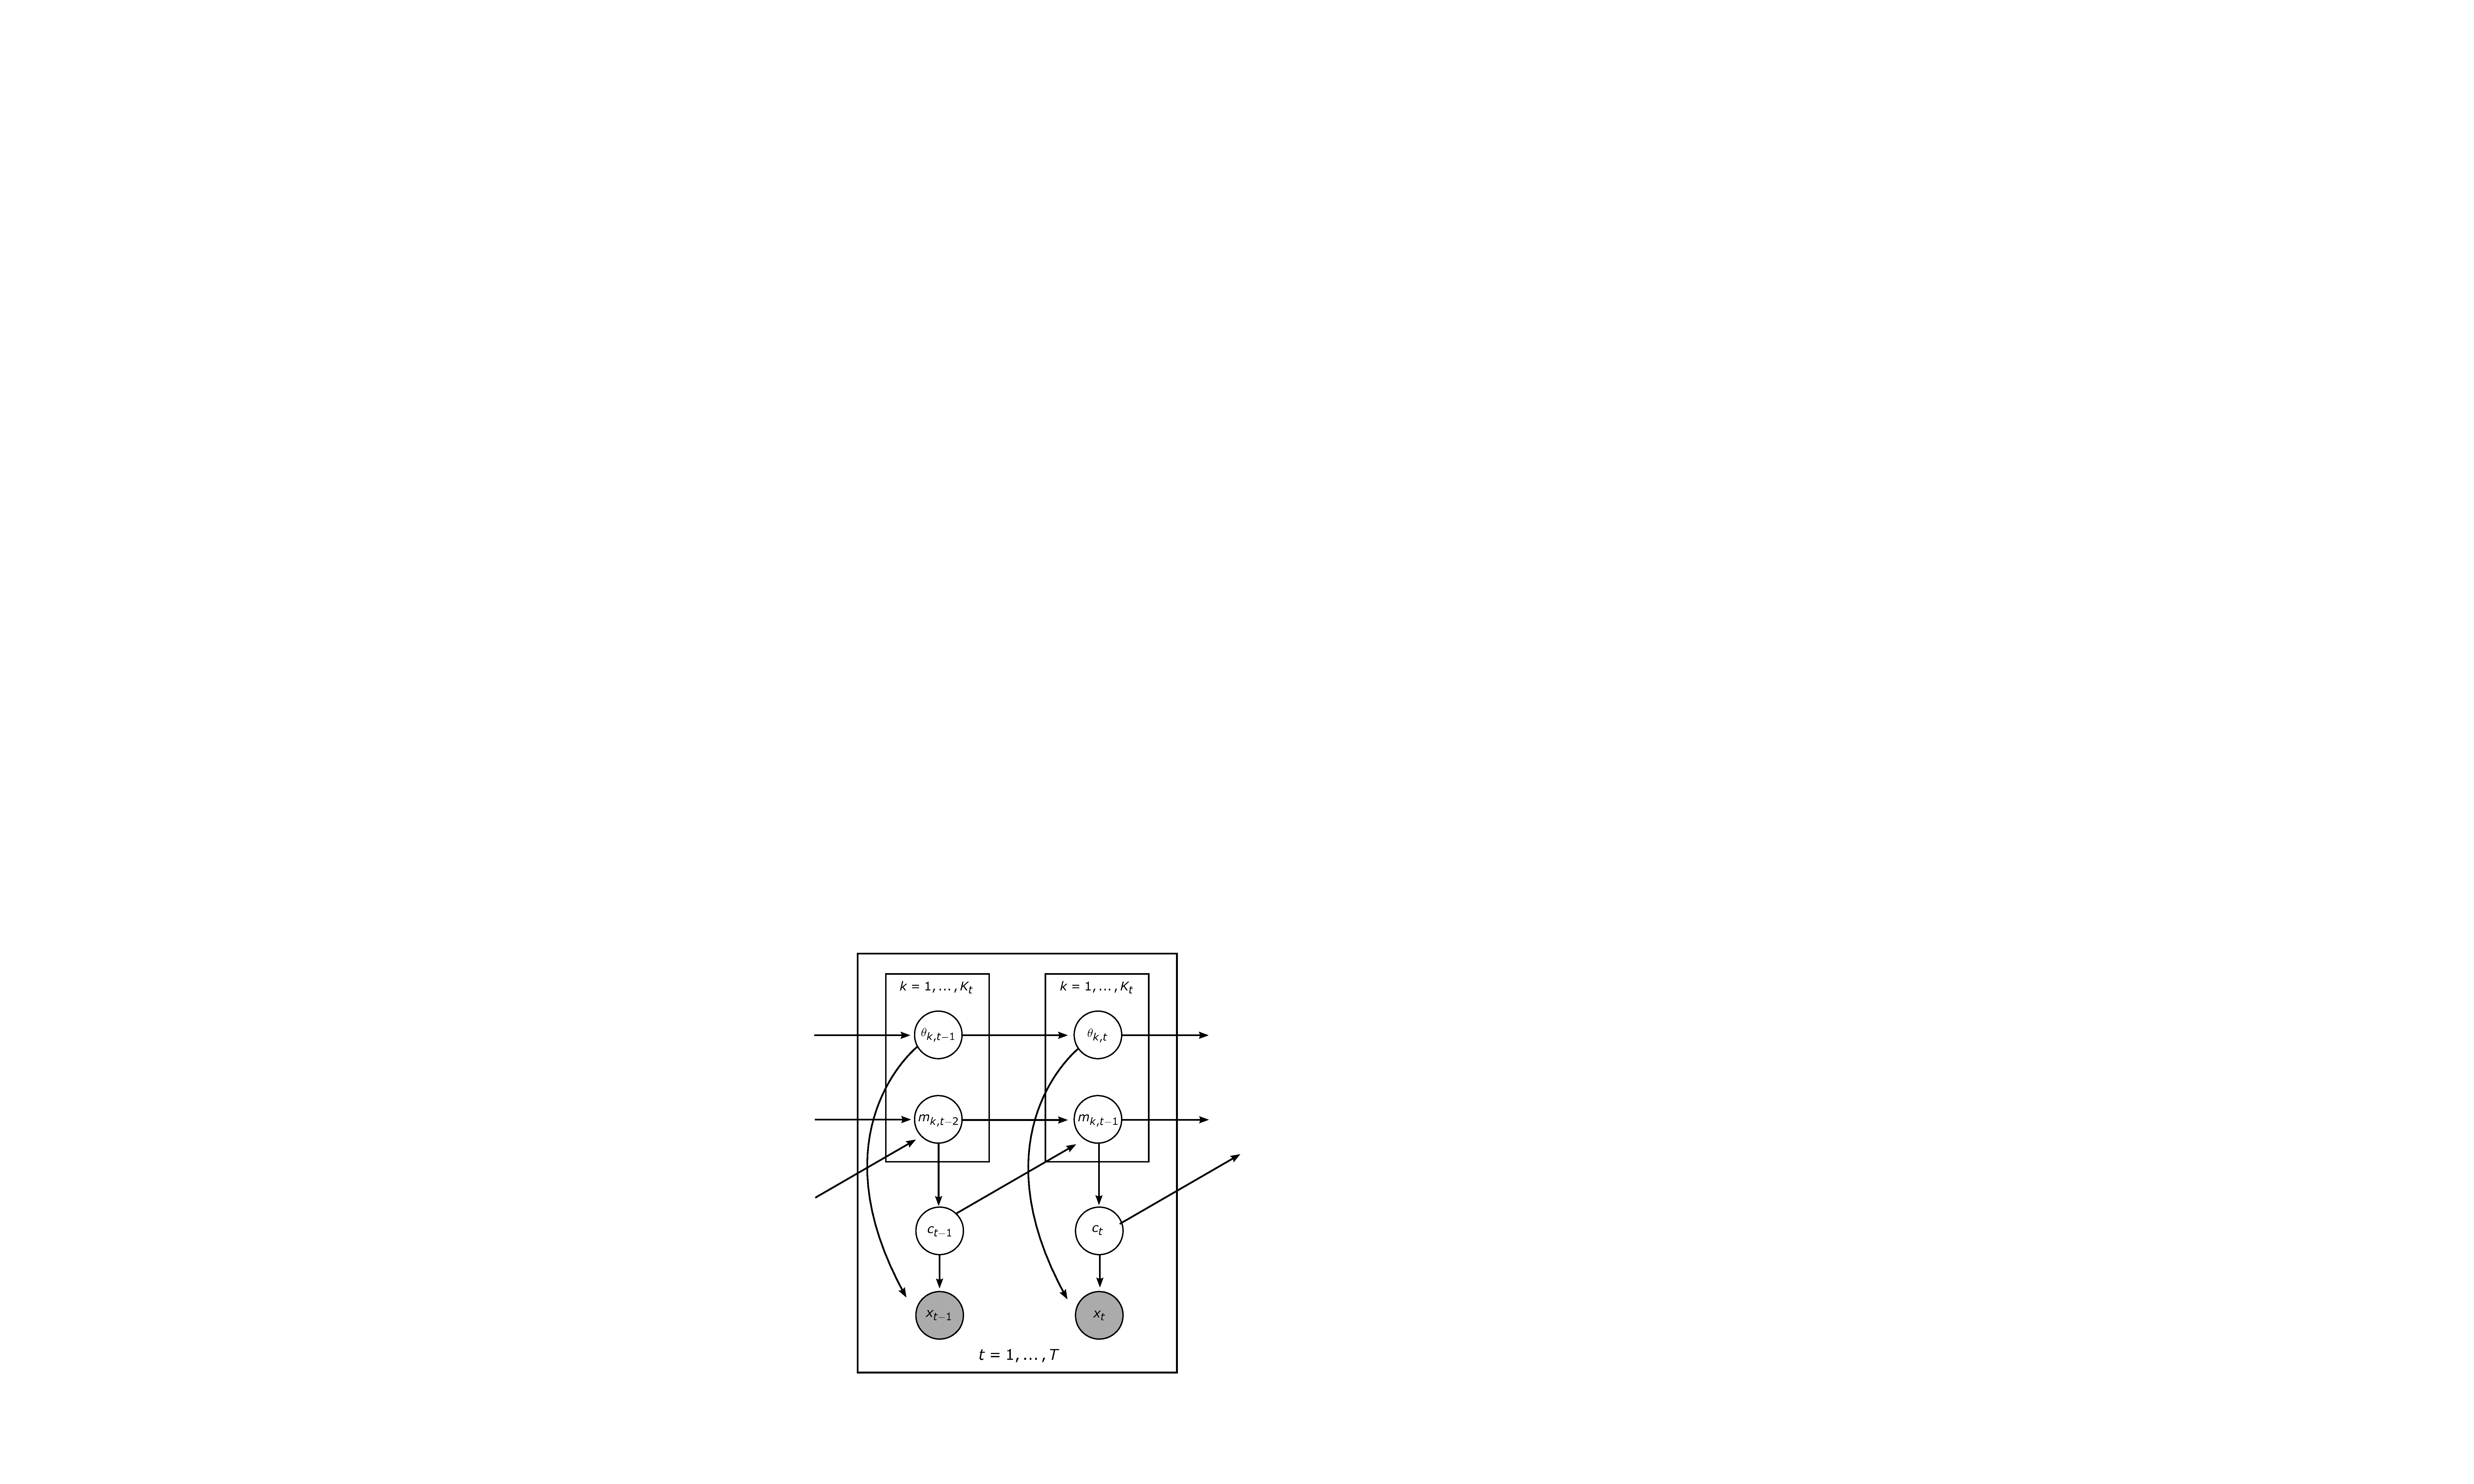
\includegraphics[width=120mm]{gpuddpm_gm_1.pdf}}
        \caption{\label{Figure 2:} Graphical Model of the Generalized Poly Urn Dependent Dirichlet Process Mixture}
\end{figure}







\subsubsection{Object Characteristics Modeled}

We would like make explicit the connection between certain elements of the GPUDDPM model and the characteristics of objects in vidoes that these elements represent.

First, the appearances of objects are moded by what we term the `likelihood and object appearance model', which we denoted by $F$. In the above modeling formulation, $F$ is the probability distribution for an observation, given that it is assigned to specified cluster (i.e. given that it is associated with a given object in a video). The likelihood and object appearance model is therefore

\begin{equation}
F(\theta_{c_{i}}) = P(x_{i}|\theta_{c_{i}})
\end{equation}

where $x_{i}$ is an observation, $c_{i}$ is its associated assignment, $\theta_{c_{i}}$ specifies the parameters of the parametric form of the $c_{i}^{th}$ cluster. The specific form of this model is dependent upon the observations $x_{i}$; recall that the observations, which as a baseline include spatial and temporal features, could include an arbitrary amount of additional features which need to be incorporated into this appearance model. A specific formulation of the appearance model can be seen in the proceeding section.

Object behavior is modeled by the dependencies between corresponding clusters at adjacent time steps. In particular, this relationship is captured by the transition kernel, $P(\theta_{k}^{t} | \theta_{k}^{t-1})$ (which captures the dependence of cluster $k$ at time $t$ on the same cluster at time $t-1$), described previously. The motion behavior of an object, i.e. the specific dependence of the parameters of cluster $k$ at a time $t$ on its parameters at time $t-1$, is therefore
\begin{equation}
Tr(\theta_{k, t} | \theta_{k, t-1}) = P(\theta_{k, t} | \theta_{k, t-1})
\end{equation}

Additionally, the base distribution $\mathbb{G}_{0}$ of the DP acts as a prior on the cluster parameters. This allows one to place a prior probability over appearances of objects. It is important that this prior is not chosen in such a specific manner that it limits this method from performing unsupervised detection of arbitrary objects.









\section{Model Specification and Inference}

In the following sections, a particular extraction method for generating data from videos and a specific formulation of the model described in Section~\ref{sec:modeloverview} are given. Inference schemes on this model, which when carried out allow for unsupervised detection and tracking of multiple arbitrary objects, are also described.



\subsection{Extraction}
\label{sec:modelspec_extraction}

We desire an extraction procedure that is as unsophisticated as possible, both to gauge the robustness of this method on potentially noisy extraction data and to ensure that the procedure is applicable to a wide range of videos. For these reasons we choose the method of frame-differencing for all extraction performed in this paper, which involves recording the positions of pixels (or pixel groups) that have exhibited differences in intensity or value in succesive frames beyond a given threshold. In particular, if we let $I_{t}$ be the image difference obtained by subtracting the value of the $(i,j)^{th}$ pixel in video frame $t$ from the value of the $(i,j)^{th}$ pixel in video frame $t+1$, we can define extraction on frame $t$ to be the process that returns the dataset
\begin{equation}
	\Omega_{t} = \{ (i,j) | I_{t}(i,j) > \phi \}
\end{equation}
where $i$ and $j$ respectively denote the two spatial positions of a pixel, and $\phi$ is a given pixel value threshold. Frame differencing on each frame $t =\{1, \ldots, T \}$ yields the dataset
\begin{equation}
	\Omega = \bigcup_{t=1}^{T} \Omega_{t} = \{ (i,j,t) | I_{t}(i,j) > \phi \}
\end{equation}
which is equivalent to data with the baseline features described in Section~\ref{sec:data}.

Frame differencing is unsophisticated, computationally inexpensive, able to be applied to a wide range of static, single-camera videos (note that videos used in the experiments described in the following sections were chosen to be static; moving-camera videos should be used in conjunction with applicable extraction methods that allow for camera movement). We have found that, when correctly implemented, frame differencing is sufficiently general to extract the desired worm-like data clouds from a variety of videos containing multiple moving objects. A few examples of this extraction procedure on single video frames can be found in Figure 3.

\begin{figure}
\centering
{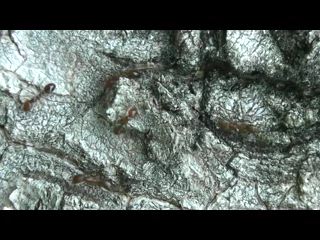
\includegraphics[width=45mm]{antpic2.png}}
%\hspace{2mm}
{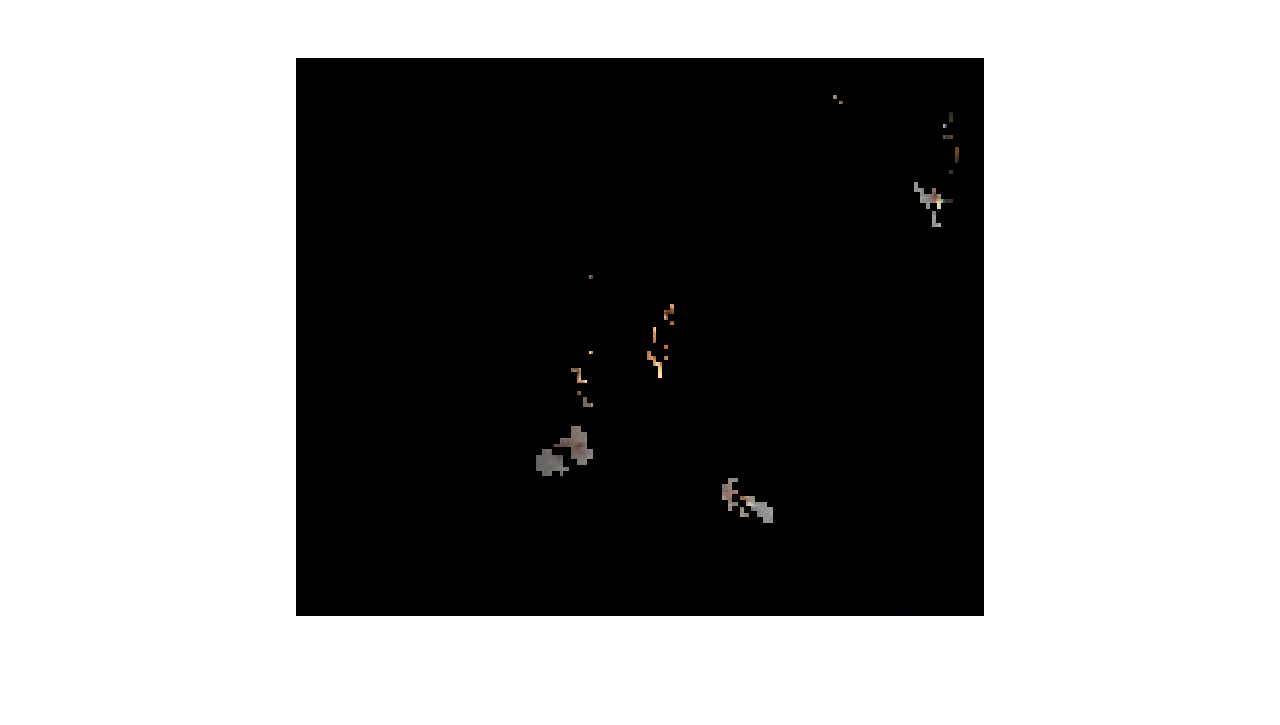
\includegraphics[width=60mm]{frame_diff_ants_1.png}}
\caption{(a.) Frame of a video containing five ants. (b.) Frame differencing extraction results from the same frame \willie{this is just a demo of the type of image i will have here... these aren't actually from the same frame, and also formatting is screwed up)}}
\label{test}
\end{figure}

We furthermore wish to capture the color (or grayscale) value of each pixel and incorporate this color information into our model. For each pixel $x = (i, j, t) \in \Omega$ (defined above), we specify a square, $L$ pixels in length, centered on $(i, j)$, that selects a set of pixels surrounding $\bold{x}$ in frame $t$. We also specify a scalar color value that is able to be computed for each pixel; this value could, for example, be some function of the r-g-b or h-s-v value of a pixel. The color value of each of the selected pixels surrounding $\bold{x}$ is recorded. Afterwards, the set of possible color values (ie the range of color values to which a pixel may be assigned) is partitioned into $V$ bins, and the number of pixels with a color value lying in each of the bins yields a $V$ dimensional vector of `color counts'. We will refer to this extraction technique as `color counting'.

\willie{Show example color-count vector (histogram) for different objects in an image. give more-formal definition like for frame differencing above.}







\subsection{Model Specification for Experiments}
%

\subsubsection{Data}

The frame differencing and color counting extraction outlined above yields a set of data $\bold{X} \subset \mathbb{R}^{2} \times \mathbb{Z}_{+}^{V} \times \mathbb{Z}_{+}$, where each element $\bold{x} \in \bold{X}$ can be written
\begin{equation}
\bold{x} = ( \bold{x}^{s}, \bold{x}^{c}, t ) = ( x^{s_{1}}, x^{s_{2}}, x^{c_{1}}, \ldots, x^{c_{V}}, t )
\end{equation}
where $\bold{x}^{s} \in \mathbb{R}^{2}$ is the two dimensional vector of spatial coordinates,  $\bold{x}^{c} \in \mathbb{Z}_{+}^{V}$ is the $V$ discrete dimensional vector of color counts, and $t \in \mathbb{Z}_{+}$ is the discrete time index. 

In the following experiments, the hue component of a pixel's h-s-v value is recorded from each pixel surrounding a given $\bold{x}^{s}$ in the manner described in Section~\ref{sec:modelspec_extraction} (where we choose $L=5$). Additionally, the set of possible hue values is partitioned into 10 bins, and the number of pixels with a hue value lying in each of the 10 bins is recorded to yield the vector of `color counts' $\bold{x}^{c} = x^{c_{1}}, \ldots, x^{c_{10}}$. Hue is chosen to represent object color since it has been demonstrated in previous work as a simple representation of object appearance that allows for distinct objects to be well differentiated (\willie{cite mckenna, other papers here}).



\subsubsection{Likelihood and Object Appearance Model}

At a given time $t$, we model each $\bold{x} \in \bold{X}$ as a draw from the product of a multivariate normal and multinomial distribution
\begin{equation}
P(\bold{x}|\theta) = \mathcal{N}(\bold{x}^{s} | \boldsymbol{\mu}, \Sigma)  \mathcal{M}n(\bold{x}^{c} | \bold{p})
\end{equation}
where $\theta = \{ \boldsymbol{\mu}, \Sigma, \bold{p} \}$ denote the parameters of a cluster at time $t$, with mean $\boldsymbol{\mu} \in \mathbb{R}^{2}$, covariance matrix $\Sigma \in \mathbb{R}^{2} \times \mathbb{R}^{2}$, and discrete probability vector $\bold{p} = (p_{1}, \ldots, p_{V})$ such that $\sum_{i=1}^{V}p_{i} = 1$. Also, $\mathcal{N}$ denotes the multivariate normal distribution and $\mathcal{M}n$ denotes the multinomial distribution, 

The distribution families assumed to generate each $\bold{x}$ must be justified. Both the multivariate normal and multinomial distributions were chosen because they are sufficiently simple (and well studied) to allow for tractable inference and sufficiently flexible to provide a reasonable approximation to the data gained during extraction. In particular, the multivariate normal distribution over the spatial features $\bold{x}^{s}$ can be thought to represent the shape of each object as an oval; likewise, data generated by each moving object during extraction are often ovular--as noisy extraction procedures cause some smoothing of edges and corners, producing blob-like shapes even when objects are not particularly round--and centered on a given object. Furthermore, this model is justified as the maximum likelihood parameter estimate of a normal distribution corresponds to the least squares fit of data relative to the mean of the distribution. \willie{needs to be said more accurately and explained why this helps.} Modeling the color features $\bold{x}^{c}$ as draws from a multinomial distribution (equivalently, as draws from a product of discrete distributions), is justified since distinct object tend to generate pixels whose hue values are noisy but yield consistent counts in discrete hue bins.



\subsubsection{Base Distribution $\mathbb{G}_{0}$ and Appearance Prior}

$\mathbb{G}_{0}$ denotes the base distribution of the time-dependent Dirichlet process mixture; it also serves as a prior distribution for the parameters $\theta = \{ \boldsymbol{\mu}, \Sigma, \bold{p} \}$ present in the likelihood. We make use of conjugate priors in the base distribution to allow for more efficient computation. Specifically, in the experiments carried out in this paper, a normal-inverse-Wishart prior is placed on the multivariate normal parameters $\{ \boldsymbol{\mu}, \Sigma \}$ , and a Dirichlet prior is placed on the multinomial parameter $ \{  \bold{p}  \} $ (where the normal-inverse-Wishart is a conjugate prior for the multivariate normal component of the likelihood and the Dirichlet is a conjugate prior for the multinomial component). The prior can thus be written
\begin{equation}
\mathbb{G}_{0}(\theta) = \mathcal{N}i\mathcal{W}(\boldsymbol{\mu}, \Sigma | \boldsymbol{\mu}_{0}, k_{0}, v_{0}, \Lambda_{0})  \mathcal{D}ir( \bold{p} | \bold{q}_{0})
\end{equation}
where $\mathcal{N}i\mathcal{W}$ denotes the normal-inverse-Wishart distribution, $\mathcal{D}ir$ denotes the Dirichlet distribution, and the prior has the hyperparameters $\boldsymbol{\mu}_{0}, k_{0}, v_{0}, \Lambda_{0}$ and $\bold{q}_{0}$.  \willie{reference text with good background on NiW and Dir distributions}



\subsubsection{Transition Kernels and Motion Behavior}

We wish to formulate a transition kernel $P(\theta_{t} | \theta_{t-1})$ that provides a reasonable representation of how we expect tracked objects to behave. In the interest of formulating a model with the intention of using it to track arbitrary objects, we do not wish to make many assumptions about the long-term behavior of objects (though transition kernels that incorporate, for example, dynamics could potentially be implemented if one is aware beforehand of an object's behavior).

As described in Section~\ref{sec:gpudpm}, $\mathbb{G}_{0}$ must be the invariant distribution of $P(\theta_{t} | \theta_{t-1})$ in order for the the cluster parameters to remain marginally distributed according to the base distribution. In other words, the transition kernel must satisfy
\begin{equation}
\int \mathbb{G}_{0}(\theta_{t-1})P(\theta_{t} | \theta_{t-1}) d\theta_{t-1} = \mathbb{G}_{0}(\theta_{t})
\end{equation}
for a given cluster $\theta$. One way to achieve this is through the use of auxiliary variables. Auxiliary variables are a set of $M$ variables $\bold{z}_{t} = (z_{t,1}, \ldots, z_{t,M})$ associated with a each cluster $\theta$ at time $t$ that satisfy
\begin{eqnarray}
% P(\theta_{k,t} | \theta_{k,t-1}) = \int P(\theta_{k,t} | \bold{z}_{k,t}) P(\bold{z}_{k,t} | \theta_{k,t-1}) d \bold{z}_{k,t}
P(\theta_{t} | \theta_{t-1}) = \int P(\theta_{t} | \bold{z}_{t}) P(\bold{z}_{t} | \theta_{t-1}) d \bold{z}_{t}  %\\
% P(\theta', \bold{z}_{t}) = p(\bold{z}_{t}|\theta') \mathbb{G}_{0}(\theta')
\end{eqnarray}

In this way, the parameters of a cluster at a given time do not depend directly on their value at the previous time; they are instead dependent upon an intermediate sequence of auxiliary variables chosen to satisfy the above criteria, which allows the cluster parameters at each time step to be marginally distributed according to the base distribution $\mathbb{G}_{0}$.

For each cluster, we introduce $M$ auxiliary variables $z_{t, 1}, \ldots, z_{t, M}$ at time $t$ that are each drawn from the product of a multivariate normal and multinomial when conditioned on the associated cluster parameters $\theta_{t} = \{ \boldsymbol{\mu}_{t}, \Sigma_{t}, \bold{p}_{t} \}$:
\begin{equation}
z_{t, m} | \boldsymbol{\mu}_{t}, \Sigma_{t}, \bold{p}_{t}  \sim  \mathcal{N}(\boldsymbol{\mu}_{t}, \Sigma_{t}) \mathcal{M}n(\bold{p}_{t})   \hspace{15pt}   
\forall m \in \{ 1, \ldots, M \}
\end{equation}
To satisfy the above criteria for auxiliary variables, at each time $t$ we specify the dependencies of a given cluster on its associated set of auxiliary variables by
\begin{equation}
\boldsymbol{\mu}_{t}, \Sigma_{t}, \bold{p}_{t} | \bold{z}_t  \sim  \mathcal{N}i\mathcal{W}(\boldsymbol{\mu}_{M}, k_{M}, v_{M}, \Lambda_{M})  \mathcal{D}ir(\bold{q}_{M})
\end{equation}
where $\boldsymbol{\mu}_{M}, k_{M}, v_{M}, \Lambda_{M},$ and $\bold{q}_{M}$ are parameters given by:
\willie{ran out of time. need to type up updates here.}




\subsection{Inference Implementations in Experiments}
%
Include a graphical model for each of the specified inference methods here? Or do I only need one graphical model for the model specified above?

Include algorithms for each of the inference procedures.










\section*{Experiments}





\subsection{Synthetic Videos}

\subsubsection{Occlusions}

\subsubsection{Similar Appearances}

\subsubsection{Different Numbers of Objects}

\subsubsection{Objects wih Diverse Characteristics}






\subsection{Real-life Videos}

\subsubsection{Complex Behavior}
%
Ants

\subsubsection{Occlusions}
%
Various people scenes

\subsubsection{Objects with Diverse Characteristics}
%
Traffic and Humans (PETS scenes)

\subsubsection{Standard Data for Comparison}
%
PETS and other standard datasets




\section*{Results and Discussion}





\section*{Conclusion}















% \begin{small}
% \bibliographystyle{plainnat}
% \bibliography{paper_refs} 
% \end{small}



\end{document}